\section{Representation}

The \textbf{Representer} takes the results of the detection module and computes a \textit{representation} of each recognized object to be tracked. In the basic tracker, the \textbf{Representer} extracts the bounding-box and size of each blob and only keeps the biggest one as the single object being tracked.

The requirements in this module was to not only extract the bounding box and the size, but also determine the velocity and a local histogram for the object being tracked.

The velocity was calculated based on the location of the \textit{centroid} of the object being tracked as follows:

\begin{equation}
velocity = (centroid - old\_centroid)% * fps
\end{equation}

%where \textit{fps} is the frames per second in the video. Therefore, in this case we have to keep the centroid of the previous object being tracked.

For the histogram, we calculated the color histogram for the object being tracked.

\begin{figure}[Color histogram]{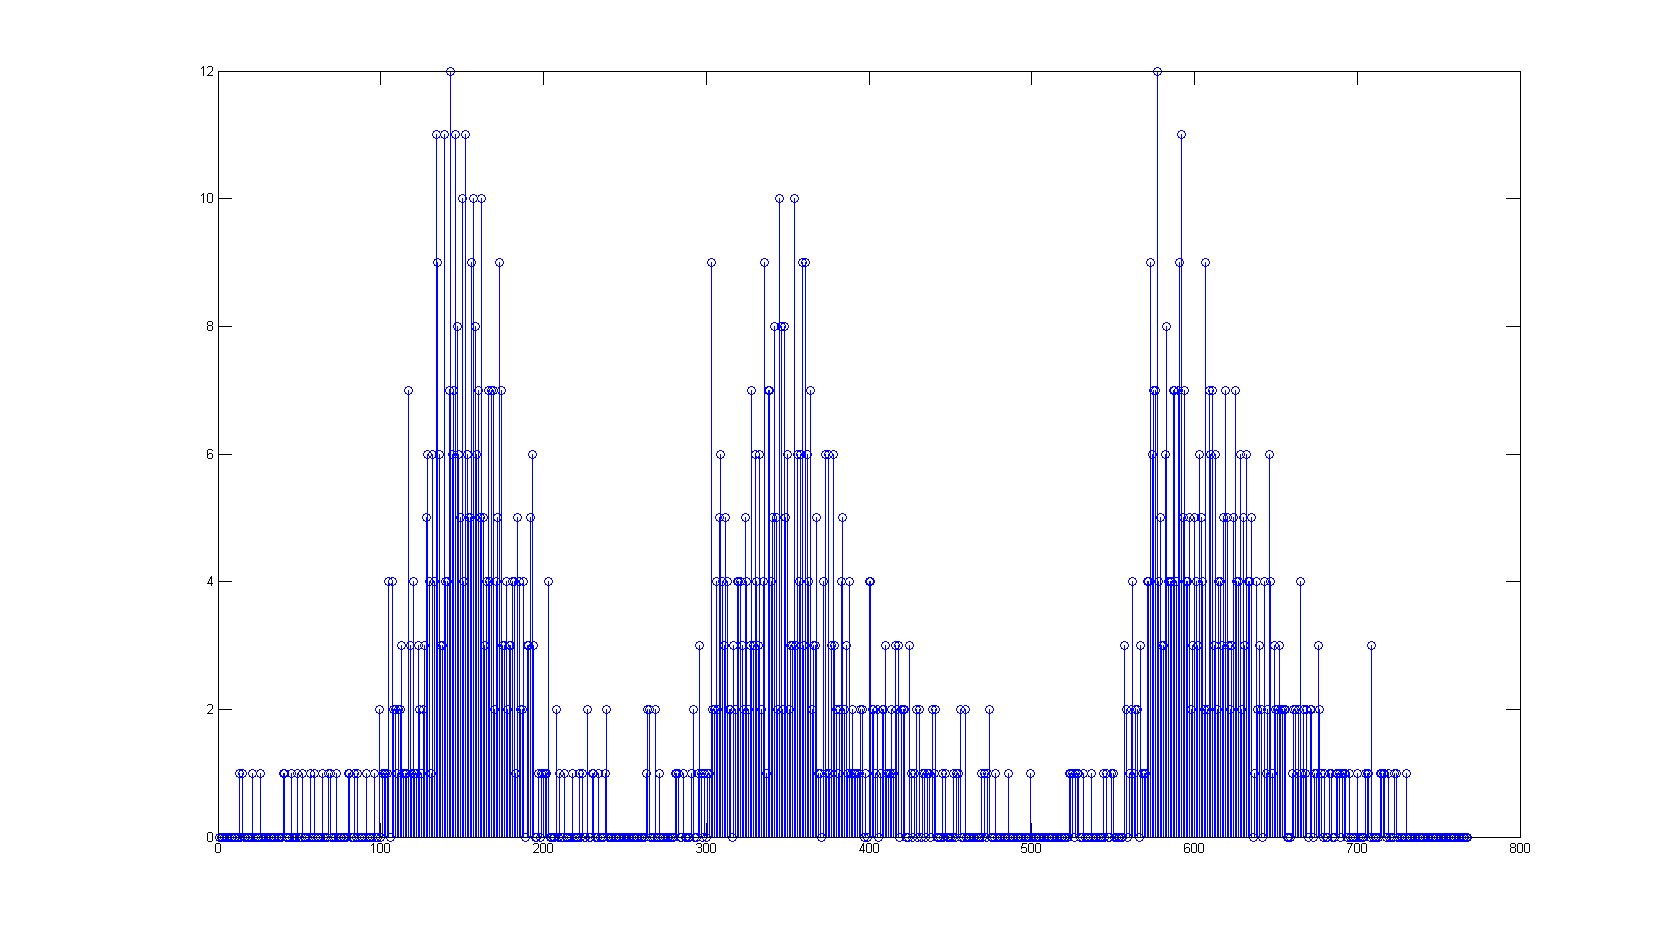
\includegraphics[width=0.9\textwidth]{histogram_car}}
  \centering
  \caption{RGB color histogram concatenated together on the same axis}
\end{figure}

According to our detection methodology. Our new \textbf{Representer} now has to solve the correspondence problem between the detected objects in different frames. There are two cases that we have to consider.

Case 1, the detector already recognized the person. In this case we don't have to do anything. The correspondence problem is already solved by the detector.

Case 2 is when the \textbf{Detector} fails to detect the face of the person. However, this person is still in the scene. We then have to find a way to correspond the blobs in the scene with the people being tracked - with a label -. We do this by getting the minimum euclidean distance between the previously prediction of the tracker for a label and the newly detected unrecognised blobs. If the closest blob is nearer than an appropriate threshold we assume that this is the new blob for the certain label. In our case the usage of the color histogram will be redundant. The colours of the faces won't be of a high discriminative power for different blobs in the scene. However, If we have implemented the person's tracker instead of a face tracker. In this case it would had been an advantage to also make use of the color histogram. Clothes of the people can be discriminative for the detected persons.
